% Document class, with margin for binding
\documentclass[	pdftex, 
                a4paper,
                oneside,
                BCOR5mm,
                12pt,
                parskip
                ]{scrbook}
%\documentclass[	pdftex, 
%                a4paper,
%                12pt, DIV11, BCOR5mm,
%                parskip,								
%                pointlessnumbers					
%                ]{scrbook}

% Mathematical packages
\usepackage{amsmath}
\usepackage{amssymb}
\usepackage{amsthm}
\usepackage{mathpartir}

% Graphical packages
\usepackage{tikz}
\usetikzlibrary{trees}
\usetikzlibrary{shapes}
\usepackage{graphicx}
\graphicspath{{./graphs/}}

% Input config
\usepackage{luatextra} % also loads fixltx2e, fontspec, xunicode
\usepackage{unicode-math}

% Font config
\setmainfont{Linux Libertine O}
\setsansfont{Linux Biolinum O}
\newfontfamily\scfont[Letters=SmallCaps]{Linux Libertine O}
\setmathfont{Latin Modern Math}
\setmonofont{Inconsolata}

% Listings, pseudo code and grammar
\usepackage{listings}
\usepackage{algpseudocode}
\algnewcommand{\LineComment}[1]{\State \(\triangleright\) #1}
\usepackage[nounderscore]{syntax}
\usepackage{float}

% References
\usepackage[nottoc,notlof,notlot]{tocbibind} % Bibliograhy in table of contents
%\usepackage{hyperref} % TODO: remove before print

% Other stuff
\usepackage{xifthen}

\begin{document}

% TUM logo
\def\oTUM#1{%
\dimen1=#1\dimen1=.1143\dimen1
\dimen2=#1\dimen2=.419\dimen2
\dimen3=#1\dimen3=.0857\dimen3
\dimen0=#1\dimen0=.018\dimen0
\dimen4=\dimen1\advance\dimen4 by-\dimen0
\setbox1=\vbox{\hrule width\dimen0 height\dimen4 depth0pt}
\advance\dimen4 by\dimen2
\setbox8=\vbox{\hrule width\dimen0 height\dimen4 depth0pt}
\advance\dimen4 by-\dimen2\advance\dimen4 by-\dimen0
\setbox4=\vbox{\hrule width\dimen4 height\dimen0 depth0pt}
\advance\dimen4 by\dimen1\advance\dimen4 by\dimen3
\setbox6=\vbox{\hrule width\dimen4 height\dimen0 depth0pt}
\advance\dimen4 by\dimen3\advance\dimen4 by\dimen0
\setbox9=\vbox{\hrule width\dimen4 height\dimen0 depth0pt}
\advance\dimen4 by\dimen1
\setbox7=\vbox{\hrule width\dimen4 height\dimen0 depth0pt}
\dimen4=\dimen3
\setbox5=\vbox{\hrule width\dimen4 height\dimen0 depth0pt}
\advance\dimen4 by-\dimen0
\setbox2=\vbox{\hrule width\dimen4 height\dimen0 depth0pt}
\dimen4=\dimen2\advance\dimen4 by\dimen0
\setbox3=\vbox{\hrule width\dimen0 height\dimen4 depth0pt}
\setbox0=\vbox{\hbox{\box9\lower\dimen2\copy3\lower\dimen2\copy5
\lower\dimen2\copy3\box7}\kern-\dimen2\nointerlineskip
\hbox{\raise\dimen2\box1\raise\dimen2\box2\copy3\copy4\copy3
\raise\dimen2\copy5\copy3\box6\copy3\raise\dimen2\copy5\copy3\copy4\copy3
\raise\dimen2\box5\box3\box4\box8}}
\leavevmode\box0}

% math commands
\newcommand{\Dmay}{Δ_\text{may}}
\newcommand{\Dmust}{Δ_\text{must}}
\newcommand{\may}[1][]{\ifthenelse{\isempty{#1}{}}
  {\dashrightarrow}
  {\stackrel{\text{#1}}{\dashrightarrow}}
}
\newcommand{\must}[1][]{\ifthenelse{\isempty{#1}}
  {\longrightarrow}
  {\stackrel{\text{#1}}{\longrightarrow}}
}
\newcommand{\attack}[1][]{\ifthenelse{\isempty{#1}}
  {\longrightarrow_a}
  {\stackrel{\text{#1}}{\longrightarrow}_a}
}
\newcommand{\call}{\text{call}}
\newcommand{\return}{\text{return}}
\newcommand{\internal}{\text{internal}}
\newcommand{\atree}{\text{ atree}}
\newcommand{\leaf}{\text{leaf}}
\newcommand{\mc}{\mathcal}

% define theorems
\theoremstyle{definition}
\newtheorem{definition}{Definition}
\theoremstyle{plain}
\newtheorem{lemma}{Lemma}
\newtheorem{theorem}{Theorem}
\newtheorem{corollary}{Corollary}
\newtheorem{example}{Example}
\theoremstyle{remark}
\newtheorem{remark}{Remark}


% tikz options
\tikzset{  
  state/.style={text centered, rectangle, draw},
  openstate/.style={text centered, rectangle, rounded corners=3mm, draw},
  attack/.style={below=-0.7em},
  label/.style={left=5.0em},
  attlabel/.style={left=14.0em},
  defense/.style={above=-0.2em},
  grow=right,
  sloped,
  edge from parent/.style={->,draw,shorten >=5pt, shorten <=5pt},
}

% listings options
\lstset{
%  breakindent=0em,
%  language=XML,
%  basicstyle=\footnotesize,
%  numbers=left,
%  numberstyle=\footnotesize,
%  stepnumber=2,
%  numbersep=5pt,
%  backgroundcolor=\color{white},
%  showspaces=false,
%  showstringspaces=false,
%  showtabs=false,
%  frame=single,
%  tabsize=2,
%  captionpos=b,
  breaklines=true,
  breakatwhitespace=true,
  breakautoindent=true,
}


% outer cover page
\pagenumbering{roman}
\thispagestyle{empty}
\begin{titlepage}
  \begin{center}
    \begin{figure}[htp]
      \centering
      \oTUM{6cm}
    \end{figure}

    \vspace*{2\baselineskip}
    
    {\large{\scfont Fakultät für Informatik}}
    
    {\large {\scfont Technische Universität München}}
    
    \vspace{1.5cm}
    
    {\large \em Bachelor's thesis in Informatics}

    {\huge Algorithms for refinement of modal process rewrite systems}

    \vspace{2.5cm}
    
    \large{Philipp Meyer}
    
    \vspace{3.0cm}
    
    \begin{figure}[htp]
      \centering
      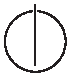
\includegraphics[width=0.20\textwidth]{IN_schwarz_CMYK.pdf}
    \end{figure}
  
  \end{center}
\end{titlepage}


% TODO look at sample if inner cover is on odd or even page
\let\cleardoublepage\clearpage

% inner cover page
\thispagestyle{empty}
\begin{titlepage}
  \begin{center}
    \begin{figure}[htp]
      \centering
      \oTUM{6cm}
    \end{figure}

    \vspace*{2\baselineskip}
    
    {\large{\scfont Fakultät für Informatik}}
    
    {\large {\scfont Technische Universität München}}
    
    \vspace{1.5cm}
    
    {\large \em Bachelor's thesis in Informatics}

    { \huge Algorithms for refinement of modal process rewrite systems}
    
    { \huge Algorithmen zur Verfeinerung von modalen Prozessersetzungssystemen}

    \vspace{1.0cm}
    \large{
      \makebox[3.5cm][l]{Author:}            \makebox[7cm][l]{\ \ \ Philipp Meyer}\\
      \makebox[3.5cm][l]{Supervisor:}        \makebox[7cm][l]{\ \ \ Univ.-Prof. Dr. Dr. h.c. Javier Esparza}\\
      \makebox[3.5cm][l]{Advisor:}           \makebox[7cm][l]{\ \ \ M. Sc. Jan Křetínský}\\
      \makebox[3.5cm][l]{Submission Date:}   \makebox[7cm][l]{\ \ \ \today}\\
    }
    
    \vspace{1.0cm}
    
    \begin{figure}[htp]
      \centering
      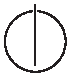
\includegraphics[width=0.20\textwidth]{IN_schwarz_CMYK.pdf}
    \end{figure}
  
  \end{center}
\end{titlepage}


\chapter*{}
  \begin{center}
    \begin{tabular}{p{12cm}}
      I assure the single handed composition of this bachelor's thesis only supported by declared resources.
      
      \vspace*{2.0em}
      
      {\em Munich, \today}
      
      \vspace*{2\baselineskip}

      \hfill
      \begin{tabular}{p{6cm}}
        \hrulefill \\
        Philipp Meyer
      \end{tabular}
    \end{tabular}
  \end{center}
\clearpage


%\chapter*{\centering \begin{normalsize}Abstract\end{normalsize}}
\begin{quotation}
\noindent % TODO abstract text
\end{quotation}
\clearpage

\begingroup

\let\cleardoublepage\relax
\let\clearpage\relax

\tableofcontents

\listoffigures % TODO remove if no tables

\listoftables

\lstlistoflistings

\endgroup


\pagenumbering{arabic}

\newpage

\chapter{Introduction}

As an extension to labeled transition systems,
modal transition systems (MTS) \cite{LarsenT88}
have been widely used, especially in model checking.
They provide a way to describe system specifications
in a way that allows stepwise refinement
and composition of several refinements.
An MTS has two types of transitions, \emph{may} transitions, which are admissible,
and \emph{must} transitions, which are necessary.
A refinement of an MTS should then still be able to perform
all must transitions and all transitions it can perform are may transitions.
This way one can gradually produce finer specifications that still conform
to the original specification, until one arrives at a concrete implementation.
Alternatively one can produce coarser specifications for abstraction.
A central problem then is to decide whether modal refinement holds between
two systems.

There are many types of MTS, 
but formalisms to describe modal transitions systems with
an infinite state space have only been explored recently \cite{BenesK12}.
For transitions systems, one powerful framework to describe them are
process rewrite systems (PRS) \cite{Mayr00, Esparza01}.
They can be used to model many widely used systems
such as pushdown automata (PDA) or Petri nets (PN).
By lifting PRS to the modal world, we obtain mPRS
and their respective modal transitions systems such as
mPDA or mPN.

Unfortunately, even for basic classes such as
stateless PDA, known as basic process algebras (BPA), already simulation is
undecidable \cite{GrooteH94}.
As refinement is a generalization of both simulation and bisimulation,
it is also undecidable on mBPA and mPDA.

However there is the subclass of visibly pushdown automata (vPDA),
which is closed under all desirable operations
and for which most problems are decidable \cite{AlurM04}.
They restrict the rules of a PDA by making visible which
actions push a symbol on a stack and which pop one.
They are still more expressive than finite automata 
and can be used to specify certain properties about the stack.
For example, they have been applied to check
parenthesis-like matching in XML streaming
\cite{KumarMV07}
and checking pre/post-conditions for module calls
in program analysis \cite{AlurEM04}.

Therefore we would like to use the modal view on vPDA
as well to allow modal specifications and abstractions.
This requires a way to test refinement between these.
Fortunately, not only simulation and bisimulation
is decidable \cite{Srba06},
but also modal refinement \cite{BenesK12}.
Based on that result, we present
an algorithm with its underlying theory
to decides modal refinement on mvPDA.




\chapter{Theory}

\section{Modal process rewrite system}

Modal process rewrite systems \cite{BenesK12} are a modal extension of process rewrite systems \cite{Mayr00, Esparza01}.
They induce a modal transition systems \cite{BenesKLS09}.

\section{Basic definitions}

\begin{definition}[Process term]

The set of process terms over a set of constants $Const$
is given by
\begin{mathpar}
  \inferrule{ }{ε ∈ \mc P}\, (0) \hspace{1cm}
  \inferrule{X ∈ Const}{X ∈ \mc P}\, (1) \\
  \inferrule{p ∈ \mc P \\ q ∈ \mc P}{p⋅q ∈ \mc P}\, (S) \hspace{1cm}
  \inferrule{p ∈ \mc P \\ q ∈ \mc P}{p\|q ∈ \mc P}\, (P)
\end{mathpar}
The processes expressions are considered modulo the usual structural congruence, i.e.
the smallest congruence such that the operator $⋅$ is associative,
$\|$ is associative and commutative and
$ε$ is a unit for both $⋅$ and $\|$.
\end{definition}

Processes that can be produced just with rule 0, 1 and S, i.e. contain no $\|$,
are called \emph{sequential processes}
and processes that can be produced just with rule 0, 1 and P, i.e. contain no $⋅$,
are called \emph{parallel processes}

\begin{definition}[Size of a process term]
  The size $|p|$ of a process term $p$ is inductively defined by
  \begin{align*}
    |ε| &= 0 \\
    |X| &= 1 \\
    |p⋅q| &= |p| + |q| \\
    |p \| q| &= |p| + |q|
  \end{align*}
  Process terms will be denoted by lowercase letters $p,q,r,s,t,…$ while single
  constants are denoted by uppercase letters $P,Q,R,S,T,…$.
  %TODO Actions are denoted by $a,b,…$.
\end{definition}

\begin{definition}[Constants of a process term]
  The set of constants $Const(p)$ appearing in a process term $p$ is inductively defined by
  \begin{align*}
    Const(ε) &= ∅ \\
    Const(X) &= \{ X \} \\
    Const(p⋅q) &= Const(p) ∪ Const(q) \\
    Const(p\|q) &= Const(p) ∪ Const(q) \\
  \end{align*}
\end{definition}

\section{Modal transition system}

Modal transition system definition from \cite{BenesK12}:
\begin{definition}[Modal transition system]
A \emph{modal transition system (MTS)} over an action alphabet $Act$ is
a triple $(\mc P, \may[], \must[])$ where $\mc P$ is a set of processes and
$\must[] ⊆ \may[] ⊆ \mc P × Act × \mc P$.
An element $(p,a,q) ∈ \may[]$ is a \emph{may transition}, also written as $p \may[a] q$,
and an element $(p,a,q) ∈ \must[]$ is a \emph{must transition}, also written as $p \must[a] q$.
\end{definition}


\section{Modal process rewrite system}

\begin{definition}[Modal process rewrite system]
A \emph{process rewrite system (PRS)} over a set of constants $Const$ and action
alphabet $Act$ is a finite relation.
$Δ ⊆ \mc P × Act × \mc P$, elements of which are called \emph{rewrite rules}.
A \emph{modal process rewrite system (mPRS)} is a tuple $(\Dmay, \Dmust)$ where
$\Dmay, \Dmust$ are process rewrite systems such that $\Dmay ⊆ \Dmust$.

An mPRS $(\Dmay, \Dmust)$ induces an MTS $(\mc P, \may[], \must[])$ as follows:
\begin{mathpar}
  \inferrule{(p, a, p') ∈ \Dmay}{p \may[a] p'} \, (1) \quad
  \inferrule{(p, a, p') ∈ \Dmust}{p \must[a] p'} \, (2) \\
  \inferrule{p \may[a] p'}{p⋅q \may[a] p⋅q} \, (3) \quad
  \inferrule{p \must[a] p'}{p⋅q \must[a] p'⋅q} \, (4) \quad
  \inferrule{p \may[a] p'}{p\|q \may[a] p\|q} \, (5) \quad
  \inferrule{p \must[a] p'}{p\|q \must[a] p'\|q} \, (6)
\end{mathpar}
\end{definition}

\section{Modal refinement}

\begin{definition}[Refinement]
  Let $(\mc P, \may, \must)$ be an MTS
  and $p,q ∈ \mc P$ be processes.
  We say that $p$ \emph{refines} $q$, written $p ≤_m q$, if there is a relation
  $\mc R ⊆ \mc P × \mc P $ such that
  $(p, q) ∈ \mc R$ and for every $(p, q) ∈ \mc R$ and every $a ∈ Act$:
  \begin{enumerate}
    \item If $p \may[a] p'$ then there is a transition $q \may[a] q'$ s.t.
          $(p',q') ∈ \mc R$.
    \item If $q \must[a] q'$ then there is a transition $p \must[a] p'$ s.t.
          $(p',q') ∈ \mc R$.
  \end{enumerate}
\end{definition}

% modal refinement of two MTS

\section{Attack tree}

\begin{definition}[Attack transition and attack tree]
  Let $(\mc P, \may, \must)$ be an MTS.
  An \emph{attack transition} is a tupel $((p,q), S)$ with $(p,q) ∈ \mc P^2 = \mc P × \mc P$
  and $S ⊆ \mc P$, also written as $(p,q) \attack_a S$.
  For $p,q ∈ \mc P$, the attack transitions are given by
  \begin{mathpar}
    \inferrule{p \may[a] p'}{(p,q) \attack_a \{ (p', q') \mid q \may[a] q' \}}
    \, (1) \hspace{1cm}
    \inferrule{q \must[a] q'}{(p,q) \attack_a \{ (p', q') \mid p \must[a] p' \}}
      \, (2) \\
  \end{mathpar}
  The set of \emph{attack trees} labeled by $s ∈ \mc P^2$ and $S ⊆ \mc P^2$ is given by
  \begin{mathpar}
    \inferrule{(p, q) \attack_a \{s_1, …, s_n\} \\ ∀ i : (s_i, T_i \atree)}
      {((p, q), (T_1, …, T_n) \atree)} \, (4)
  \end{mathpar}
  
  For each state $(p,q) ∈ \mc A$ we can construct a rooted and labeled \emph{attack tree}
  by setting the root to $(p,q)$, labeling it with $(p,q) \attack_a S$ and setting
  the set of successors to the trees of states $(p',q') ∈ S$.

  %TODO rewrite
  Intuitively, an attack transition $(p,q) \attack_a S$ means that from  
  the state $(p,q)$, there is a sequence of \emph{attack transitions}, that is 
  a may transition from the left side or a must transition from the right side,
  such that $S$ is the set of reachable states by applying
  appropriate \emph{defending transition}, that is a transition of the same type and
  with the same action symbol from the other side.
\end{definition}

\begin{theorem}
  \label{theorem:attack-refinement}
  For an MTS $(\mc P, \may, \must)$ and processes $p,q ∈ \mc P$:
  \[
    (p ≤_m q) \iff ¬∃ T : ((p,q), T \atree)
  \]
\end{theorem}

\begin{proof}
    \Rightarrow: Assume $p ≤_m q$. Then there is a refinement relation $\mc R$.
      Assume there is an attack tree $((p, q), T \atree)$.
      We show that any $((p,q), T)$ that $(p, q) ∉ R$
      by induction on the attack tree:
      \begin{enumerate}
        \item $T = ()$. Then there is an attack transition $(p, q) \attack_a ∅$.
          Contradiction.
        \item $T = (T_1, …, T_n)$. Then $(p, q) \attack_a (s_1, …, s_2)$.
          By refinement there is an $s_i ∈ \mc R$. But as $(s_i, T_i \atree)$
          the induction hypothesis gives $s_i ∉ \mc R$ resulting in a contradiction.
      \end{enumerate}
      So for $(p,q)$ there is no attack tree.

    \Leftarrow: Assume $¬∃ T : ((p,q), T \atree)$
      We show that $\mc R := \{ (p,q) \mid ¬∃ T : ((p,q), T \atree \}$ is a valid
      refinement relation. First $(p,q) ∈ \mc R$, and for any $(p,q) ∈ \mc R$:
      \begin{enumerate}
        \item If $p \may[a] p'$, then
            by inference rule 1 there exists $(p,q) \attack_a S$.
            From all $(p,q) \attack_a S$, choose the one where $S$ is minimal
            with regard to the inclusion order.
            There exists $(p',q') ∈ S : ¬∃ T' : ((p',q'), T' \atree)$, because otherwise
            there would be a $((p,q), T \atree)$. So this
            $(p', q') ∈ S$ was created from a transition $q \may[a] q'$ and we have
            $(p', q') ∈ \mc R$
        \item If $q \must[a] q'$, by similiar argument we get a transition
          $p \must[a] p'$ for which $(p',q') ∈ \mc R$.
      \end{enumerate}
      With this refinement relation we have $p ≤_m q$.
\end{proof}

\section{Visibly pushdown automaton}

\begin{definition}[Visibly pushdown automaton]
A PRS is a visibly pushdown automaton (vPDA) if
all processes are sequential and there is a partition
$Act = Act_r \uplus Act_i \uplus Act_c$
such that each rule $(p, a, p') ∈ Δ$ has the form
\begin{align*}
  p &= P⋅S
  & &\text{and} &
  p' &= \begin{cases}
  Q & \text{if } a ∈ Act_r \quad \text{(return rule)}\\
  Q⋅T & \text{if } a ∈ Act_i \quad \text{(internal rule)} \\
  Q⋅T⋅R & \text{if } a ∈ Act_c \quad \text{(call rule)}
\end{cases}
\end{align*}
The modal extension for a \emph{modal visibly pushdown automaton (mvPDA)} is straightforward.
\end{definition}

\begin{definition}[Attack rules for mvPDA]
  Let $(\Dmay, \Dmust)$ be an mvPDA.
  We define a \emph{attack rules} $(p,q) \attack_b S$  obtainable from the rewrite rules.
  For every $p,q ∈ \mc P$, we have:
  \begin{mathpar}
    \inferrule{(p, a, p') ∈ \Dmay}{(p,q) \attack_b \{ (p', q') \mid (q, a, q') ∈ \Dmay \}}
      \, (1) \\
    \inferrule{(q, a, q') ∈ \Dmust}{(p,q) \attack_b \{ (p', q') \mid (p, a, p') ∈ \Dmust \}}
      \, (2) \\
    \inferrule{(p,q) \attack_b \{(p'⋅P,q'⋅Q)\} \uplus S \\ (p',q') \attack_b S' \\
      ∀(p'',q'') ∈ S' : |p''| ≤ 2 }
      {(p,q) \attack_b S ∪ \{  (p''⋅P, q''⋅Q) \mid (p'',q'') ∈ S' \}} \, (3) \\
    \inferrule{(p,q) \attack_b \{(p',q')\} \uplus S \\ (p',q') \attack_b S' \\
      ∀(p'',q'') ∈ S' : |p''| ≤ 2 }
      { (p,q) \attack_b S ∪ S'} \, (4)
  \end{mathpar}
\end{definition}

%TODO Rule righthandside
%TODO Rule lefthandside

Due to the conditions on the rewrite rules of an mvPDA and the construction of the
attack rules, we can see
that for any element $(p,q) \attack_b S$ it holds that
$|p| = |q| = 2$ and for any $(p',q') ∈ S$ that $1 ≤ |p'| = |q'| ≤ 3$.

\begin{lemma}
  \label{lemma:attack-extension}
  For an MTS generated by a mvPDA, if $(p, q) \attack_a S$, then
  $(p⋅s,q⋅t) \attack_a S'$ with $S' = \{ (p'⋅s,q'⋅t) \mid (p', q') ∈ S\}$
  for any $s,t ∈ \mc P$.
\end{lemma}
\begin{proof}
  By the MTS induction rules, we have that for
  every $p \may[a] p'$ is generated from a $(p, a, p') ∈ \Dmay$
  and for a mvPDA therefore $|p| = 2$. Then there is only one transition from $p⋅s$,
  nameley $p⋅s \may[a] p'⋅s$ generated by the MTS induction rule 1.
  Also for every $q \must[a] q'$ there is just $q⋅t \may[a] q'⋅t$ from $q⋅t$.
  
  % TODO update
      Then it is a single transition created from $p \may[a] p'$
      with $S = \{ (p', q') \mid q \may[a] q' \}$ and we get
      $p⋅s \may[a] p'⋅s$ and $\{ (p'⋅s, q'⋅t) \mid q⋅t \may[a] q'⋅t \} = S'$.
      If the transition was created from $q \must[a] q'$
      with $S = \{ (p', q') \mid p \must[a] p' \}$ and we get
      $\{ (p'⋅s, q'⋅t) \mid p⋅t \must[a] p'⋅t \} = S'$
      Both cases yield $(p⋅s,q⋅t) \attack_a^* S'$.
\end{proof}

\begin{theorem}
  For an mvPDA $(\Dmay, \Dmust)$ with its induced MTS $(\mc P, \may[], \must[])$,
  it holds that for any $P,S,Q,R ∈ Const$:
  \[
    ∃ T ((P⋅S,Q⋅R), T \atree) \iff (P⋅S,Q⋅T) \attack_b ∅
  \]
\end{theorem}
\begin{proof}
    \Rightarrow: Assume $((P⋅S,Q⋅T), T \atree)$ and let $(a_1, a_2, …, a_n)$ be
      the linear form of a derivation of the attack sequence. Always
      $a_1$ has the form $(P⋅S, Q⋅R) \attack_a S$ and $a_n$ the form
      $(p,q) \attack_a ∅$.

      Our proposition is that if we can split up the sequence into subsequences
      which we can all compute seperately, we can also compute the whole sequence.
      More formally, we want to show that if there is a
      set of $k+1$ indices $I = {i_0,…,i_k}$ where
      \begin{enumerate}
        \item $0 = i_0 < i_1 < i_2 < … < i_{k-1} < i_k = n$.
        \item There is a sequence $(b_1, …, b_k)$ where
          each $b_i$ is an attack rule $(p,q) \attack_b S$.
        \item For every $i,j ∈ I$ with $i<j$ the sequence $(a_{i+1},…,a_j)$, which
          generates the attack sequence $(p,q) \attack_a^* S$, the representing rule
          $b_j$ is $(p,q) \attack_b S$
          If $j < n$ then with $b_i = (p',q') \attack_b S'$ we require $(p',q') ∈ S'$.
          and if $j = n$ then $S = ∅$.
      \end{enumerate}
      there is $(P⋅S,Q⋅T) \attack_b ∅$.

      We prove this by induction on the number $k$:

      \begin{enumerate}
        \item $k=1$: Then the indices are $0, n$ and the rule sequence $(b_1)$
          represents $(a_1, …, a_n)$ generating $(P⋅S, Q⋅T) \attack_a^* ∅$.
          Then we have $(P⋅S, Q⋅T) \attack_b ∅$.
        \item $k > 1$, and the induction hypothesis holds for any $k' < k$:
          Let $(b_1, …, b_k)$ be the rule sequence.
          For the first rule $b_1 = (P⋅S,Q⋅T) \attack_b S$, there
          is be $(p',q') ∈ S$ with $|p'| = |q'| ≥ 2$ because otherwise no more rules
          could be applied afterwards, in contradiction to $k > 1$.
          So this is a left-hand side rule.
          Also the last rule $b_k = (p',q') \attack_b ∅$ is a right-hand side rule.
          %
      \end{enumerate}
    \Leftarrow:
      We show that for $(p,q) \attack_b ∅$, there is $((p,q), T \atree)$
      by induction on the inference of
      $(p,q) \attack_b S$:
      \begin{enumerate}
        \item It was created by rule 1 from $(p, a, p') ∈ \Dmay$. Then there is
          $p \may[a] p'$.
          For every $(q, a, q') ∈ \Dmay$ there is $q \may[a] q'$ and for every
          $q \may[a] q''$ it follows that $q' = q''$.
          Then $\{ (p', q') \mid q \may[a] q' \} = S$ and
          $(p, q) \attack_a^* S$.
        \item It was created by rule 2 from $(q, a, q') ∈ \Dmust$. Then there is
          $q \may[a] q'$.
          For every $(p, a, p') ∈ \Dmay$ there is $p \may[a] p'$ and for every
          $p \may[a] p''$ it follows that $p' = p''$.
          Then $\{ (p', q') \mid p \may[a] p' \} = S$ and
          $(p, q) \attack_a^* S$.
        \item It was created by rule 3 from $(p,q) \attack_b \{(p'⋅P,q'⋅Q)\} \uplus S'$ and
          $(p',q') \attack_b S''$ with $S = S' ∪ S'''$ for $S''' = \{  (p''⋅P, q''⋅Q) \mid (p'',q'') ∈ S'' \}$
          Then by induction hypothesis there is $T' ⊆ \{(p'⋅P,q'⋅Q)\} \uplus S'$ with
          $(p,q) \attack_a^* T'$ and $T'' ⊆ S''$ with $(p',q') \attack_a^* T''$.
          If $(p'⋅P,q'⋅Q) ∉ T'$, then we get $T' ⊆ S' ⊆ S$.
          If $(p',q') ∈ T'$, with lemma \ref{lemma:attack-extension} we have
          regard the $(p'⋅P,q'⋅Q) \attack_a^* T'''$ with $T''' ⊆ S'''$.
          Then with lemma \ref{lemma:attack-associativity} we get
          that there is $T ⊆ T' ∖ \{(p',q'\} ∪ T''' ⊆ S' ∪ S''' = S$ with $(p,q) \attack_a^* T$.
        \item It was created by rule 4 from $(p,q) \attack_b \{(p',q')\} \uplus S$ and
          $(p',q') \attack_b S'$ with $S ∪ S' = ∅$, therefore $S = ∅$ and $S' = ∅$.
          Then by induction hypothesis we get $T'$ with $(p',q'), T' \atree$.
          $(p,q) \attack_a^* T'$ and $T'' ⊆ S''$ with $(p',q') \attack_a^* T''$.
          If $(p',q') ∉ T'$, then we get $T' ⊆ S' ⊆ S$.
          If $(p',q') ∈ T'$, then with lemma \ref{lemma:attack-associativity} we get
          that there is $T ⊆ T' ∖ \{(p',q'\} ∪ T'' ⊆ S' ∪ S'' = S$ with $(p,q) \attack_a^* T$.
      \end{enumerate}
      Then if $(P⋅S,Q⋅T) \attack_b ∅$ we have $(P⋅S,Q⋅T) \attack_a^* ∅$
\end{proof}

% theory and background


\chapter{The algorithm}

\section{Description}

\section{Implementation}

% pseudocode
\begin{figure}[ht]
\caption{Algorithm for calculating the attack rules on mvPDAs}
\begin{algorithmic}[1]
\Function{AttackRules}{$mvPDA = (\Dmay, \Dmust)$}
  \State $rules ← ∅$
  \For{$P,Q,S,T ∈ Const(mvPDA), a ∈ Act(mvPDA), type ∈ \{\text{may},\text{must}\}$}
    \If{$type = \text{may}$}
      \State $lhs ← (P⋅S, Q⋅T)$
      \Comment{Attack from left-hand side for may rules}
    \Else
      \State $lhs ← (Q⋅S, P⋅Y)$
      \Comment{Attack from right-hand side for must rules}
    \EndIf
    %\State $lhs ← (p, q)(X, Y)$
    \For{$(P⋅S, a, p') ∈ Δ_{type}$}
      \State $rhs ← ∅$
      \For{$(Q⋅T, a, q') ∈ Δ_{type}$}
        \If{$type = \text{may}$}
          \State $newRhs ← (p', q')$
        \Else
          \State $newRhs ← (q', p')$
        \EndIf
        \State $rhs ← rhs ∪ \{ newRhs \}$
      \EndFor
      \State $rules ← rules ∪ \{(lhs, rhs)\}$
    \EndFor
  \EndFor
  \State \textbf{return} $rules$
\EndFunction
\end{algorithmic}
\end{figure}

\begin{figure}[ht]
\caption{Algorithm for combining attack rules}
\begin{algorithmic}[1]
  \Function{Combine}{$lhsRule = (lhs, lhsRhsSet), rhsRule = (rhsLhs, rhsSet)$}
  \State $rules ← ∅$
  \If{$\forall rhs ∈ rhsSet : size(rhs) ≤ 1$}
    \For{$lhsRhs ∈ lhsRhsSet : lhsRhs = rhsLhs⋅p$}
      \State $newRhs ← (lhsRhsSet ∖ lhsRhs) ∪ \{ rhs⋅p \mid rhs ∈ rhsSet \}$
      \State $rules ← rules ∪ \{ (lhs, newRhs) \}$
    \EndFor
  \EndIf
  \State \textbf{return} $rules$
\EndFunction
\end{algorithmic}
\end{figure}

\begin{figure}[ht]
\caption{Refinement algorithm for mvPDAs}
\begin{algorithmic}[1]
\Function{VPDARefinement}{$P⋅S, Q⋅T, mvPDA$}
  \Comment{$P⋅S ≤_m Q⋅T$ given $mvPDA$}
  \State $initial ← [P⋅S, Q⋅T]$
  \State $rules ← \Call{AttackRules}{mvPDA}$
  \While{$\exists lhsRule, rhsRule ∈ rules :
      \Call{Combine}{lhsRule, rhsRule} ⊄ rules $}
    \State $rules ← rules ∪ \Call{Combine}{lhsRule, rhsRule}$
  \EndWhile
  \State \textbf{return} $(initial, ∅) ∈ rules$
\EndFunction
\end{algorithmic}
\end{figure}

\section{Soundness and completeness}

Follows from theorem \label{theorem:refinement-tree} and
theorem \label{theorem:tree-attack} and

% proof: no refinement => algorithm outputs false
% proof: algorithm outputs false => no refinement
% termination proof
% termination proof

\section{Runtime}

% tests with complete number

\section{Optimizations}

% only keep smallest rhs rules

% exploration of reachable states

% hash map for looking up lhs/rhs

% early stopping

\section{Input and output}

% now command line
% future integration with gui
% similiar input file to existing programs

\section{Performance evaluation}

\section{Example}

Figure \ref{mvpda-p} and \ref{mvpda-q} define two mvPDA. The corresponding may transitions for the must transitions are implied.
The problem is to decide whether $p⋅S ≤_m q⋅S$.

\begin{figure*}[ht]
  \centering
  \begin{minipage}[b]{.4\textwidth}
    \begin{align*}
      P⋅S &\must[coin] P⋅M⋅S \\
      P⋅M &\must[coin] P⋅M⋅M \\
      P⋅M &\must[tea] T \\
      P⋅M &\must[coffee] c \\
      T⋅M &\must[tea] T \\
      T⋅S &\must[coin] P⋅M⋅S \\
      c⋅M &\must[coffee] c \\
      c⋅S &\must[coin] P⋅M⋅S
    \end{align*}
    \caption{mvPDA for process $P⋅S$}\label{mvpda-p}
  \end{minipage}\qquad
  \begin{minipage}[b]{.4\textwidth}
    \begin{align*}
      Q⋅S &\may[coin] Q⋅T⋅S \\
      Q⋅S &\may[coin] Q⋅C⋅S \\
      Q⋅T &\may[coin] Q⋅T⋅T \\
      Q⋅C &\may[coin] Q⋅C⋅C \\
      Q⋅T &\must[tea] Q \\
      Q⋅T &\may[coffee] Q \\
      Q⋅C &\may[tea] Q \\
      Q⋅C &\must[coffee] Q
    \end{align*}
    \caption{mvPDA for process $Q⋅S$}\label{mvpda-q}
  \end{minipage}
\end{figure*}

\begin{figure*}[ht]
  \centering
\begin{tikzpicture}[
  level 1/.style={level distance=6cm, sibling distance=3.5cm},
  level 2/.style={level distance=8cm, sibling distance=2cm},
  level 3/.style={level distance=7cm, sibling distance=2cm},
  edge from parent path={(\tikzparentnode.east) -- (\tikzchildnode.west)},
  scale=0.6,
  every node/.style={scale=0.6}
]
\node[state] {$(p⋅S,q⋅S)$}
    child {
        node[state] {$(p⋅M⋅S,q⋅T⋅S)$}
        child {
          node[state] {$(p⋅M⋅M⋅S,q⋅T⋅T⋅S)$}
          child {
            node[state] {$(c⋅M⋅T,q⋅T⋅S)$}
            node[attack] {$q⋅T \must[tea] q $}
            edge from parent
            node[defense] {$q⋅T \may[coffee] q $}
          }
          node[attack] {$p⋅M \may[coffee] c $}
          edge from parent
          node[defense] {$q⋅T \may[coin] q⋅T⋅T $}
        }
        node[attack] {$p⋅M \may[coin] p⋅M⋅M $}
        edge from parent
        node[defense] {$q⋅S \may[coin] q⋅T⋅S $}
    }
    child {
        node[state] {$(p⋅M⋅S,q⋅C⋅S)$}
        child {
          node[state] {$(p⋅M⋅M⋅S,q⋅C⋅C⋅S)$}
          child {
            node[state] {$(T⋅M⋅S,q⋅C⋅S)$}
            node[attack] {$q⋅C \must[coffee] q $}
            edge from parent
            node[defense] {$q⋅C \may[tea] q $}
          }
          node[attack] {$p⋅M \may[tea] T $}
          edge from parent
          node[defense] {$q⋅C \may[coin] q⋅C⋅C $}
        }
        node[attack] {$p⋅M \may[coin] p⋅M⋅M $}
        edge from parent
        node[defense] {$q⋅S \may[coin] q⋅C⋅S $}
    }
    node[attack] {$p⋅S \may[coin] p⋅M⋅S $}
    ;
\end{tikzpicture}
  \caption{Tree for winning strategy}\label{pq-tree}
\end{figure*}

\begin{figure*}[ht]
  \centering
\begin{tikzpicture}[
  level 1/.style={level distance=2cm, sibling distance=4cm},
  level 2/.style={level distance=8cm, sibling distance=2cm},
  level 3/.style={level distance=6cm, sibling distance=2cm},
  northchild/.style={edge from parent path={(\tikzparentnode.north) -- (\tikzchildnode.south)}},
  southchild/.style={edge from parent path={(\tikzparentnode.south) -- (\tikzchildnode.north)}},
  rightchild/.style={edge from parent path={(\tikzparentnode.east) -- (\tikzchildnode.west)}},
  scale=0.6,
  every node/.style={scale=0.6}
]
\node[state] {$(p⋅S,q⋅S) \attack[] \{ (p⋅M⋅S,q⋅C⋅S), (p⋅M⋅S,q⋅T⋅S) \}$}
    child[southchild] {
      node[state] {$(p⋅M,q⋅T) \attack[] \{ (p⋅M⋅M,q⋅T⋅T) \}$}
        child[rightchild] {
          node[state] {$(p⋅M,q⋅T) \attack[] \{ (c,q) \} $}
          child[rightchild] {
            node[state] {$(c⋅M,q⋅T) \attack[] ∅$}
            edge from parent
            node[defense] {return}
          }
          edge from parent
          node[defense] {call}
        }
        edge from parent
        node[defense] {call}
    }
    child[northchild] {
      node[state] {$(p⋅M,q⋅C) \attack[] \{ (p⋅M⋅M,q⋅C⋅C) \}$}
        child[rightchild] {
          node[state] {$(p⋅M,q⋅C) \attack[] \{ (T,q) \} $}
          child[rightchild] {
            node[state] {$(T⋅M,q⋅C) \attack[] ∅$}
            edge from parent
            node[defense] {return}
          }
          edge from parent
          node[defense] {call}
        }
        edge from parent
        node[defense] {call}
    }
    ;
\end{tikzpicture}
  \caption{Tree for winning strategy with attack rules}\label{pq-attack-tree}
\end{figure*}

\begin{figure*}[ht]
  \centering
\begin{tikzpicture}[
  level 1/.style={level distance=10cm, sibling distance=4cm},
  level 2/.style={level distance=8cm, sibling distance=2cm},
  state/.style={text centered, rectangle, draw},
  edge from parent path={(\tikzparentnode.east) -- (\tikzchildnode.west)},
  scale=0.6,
  every node/.style={scale=0.6}
]
\node[state] {$(p⋅S,q⋅S) \attack[] \{ (p⋅M⋅S,q⋅C⋅S), (p⋅M⋅S,q⋅T⋅S) \}$}
    child {
      node[state] {$(p⋅M,q⋅T) \attack[] \{ (c⋅M,q⋅T) \}$}
        child {
          node[state] {$(c⋅M,q⋅T) \attack[] ∅$}
          edge from parent
          node[defense] {internal}
        }
        edge from parent
        node[defense] {call}
    }
    child {
      node[state] {$(p⋅M,q⋅C) \attack[] \{ (T⋅M,q⋅C) \}$}
        child {
          node[state] {$(T⋅M,q⋅C) \attack[] ∅$}
          edge from parent
          node[defense] {internal}
        }
        edge from parent
        node[defense] {call}
    }
    ;
\end{tikzpicture}
  \caption{Merged tree for winning strategy with attack rules after one step}\label{pq-attack-tree-1}
\end{figure*}


\begin{figure*}[ht]
  \centering
\begin{tikzpicture}[
  level 1/.style={level distance=12cm, sibling distance=4cm},
  edge from parent path={(\tikzparentnode.east) -- (\tikzchildnode.west)},
  scale=0.6,
  every node/.style={scale=0.6}
]
\node[state] {$(p⋅S,q⋅S) \attack[] \{ (p⋅M⋅S,q⋅C⋅S), (p⋅M⋅S,q⋅T⋅S) \}$}
    child {
      node[state] {$(p⋅M,q⋅T) \attack[] ∅$}
        edge from parent
        node[defense] {call}
    }
    child {
      node[state] {$(p⋅M,q⋅C) \attack[] ∅$}
        edge from parent
        node[defense] {call}
    }
    ;
\end{tikzpicture}
  \caption{Merged tree for winning strategy with attack rules after two steps}\label{pq-attack-tree-2}
\end{figure*}


\begin{figure*}[ht]
  \centering
\begin{tikzpicture}[
  edge from parent path={(\tikzparentnode.east) -- (\tikzchildnode.west)},
  scale=0.6,
  every node/.style={scale=0.6}
]
\node[state] {$(p⋅S,q⋅S) \attack[] ∅$};
\end{tikzpicture}
  \caption{Final merged tree for winning strategy}\label{pq-attack-tree-3}
\end{figure*}

\chapter{Conclusion}

\section{Main results}

In this thesis, an algorithm for deciding modal refinement
between modal visibly pushdown automata was presented.
This was done by use of modal process rewrite systems
and a new representation of refinement by attack trees.

The theoretical part introduced the concepts and showed
correctness of the construction.
The practical part described the implementation,
including some optimizations, and analyzed the
complexity with theoretical bounds and a performance evaluation.
This showed the unavoidable exponential runtime and
conditions on input which produce or avoid it.

This will hopefully contribute to the usage of mvPDA
in the fields applying modal transitions systems, such as in
system specifications and model checking, by providing
a sound and complete way to test refinement.

\section{Further extensions}

Even with the exponential runtime, there is certainly
still room for more optimizations to improve the runtime.
One possibility would be deciding positive refinement in certain cases before
exploring the whole rule space, for example by showing that there are
loops from each attack transition.
It should also be possible reduce the worst-time complexity
to $2^{\mathcal O(n^2)}$ instead of $2^{\mathcal O(n^6)}$.

Further algorithms to decide 
refinement between other classes of mPRS could be developed,
at least where it is possible, for example
between finite mFSM and general mPRS \cite{BenesK12}. Also there could be a
specialized algorithm for mvBPA, for which the refinement is PTIME-complete.

The tool also still needs to be integrated into the MoTraS system to be made
available for end users. Then more options could be added, for example
more verbose output such as optionally providing a counterexample
in case of negative refinement.



\bibliographystyle{amsalpha}
\bibliography{main}

\end{document}
